% !TeX root = ../../main.tex
\section{Mechanical drawings}
\label{app:reactor-drawings}
\subsection{3D mechanical design and engineering drawings}
\label{app:engineeringdesign}

\begin{figure}[H]
    \centering
    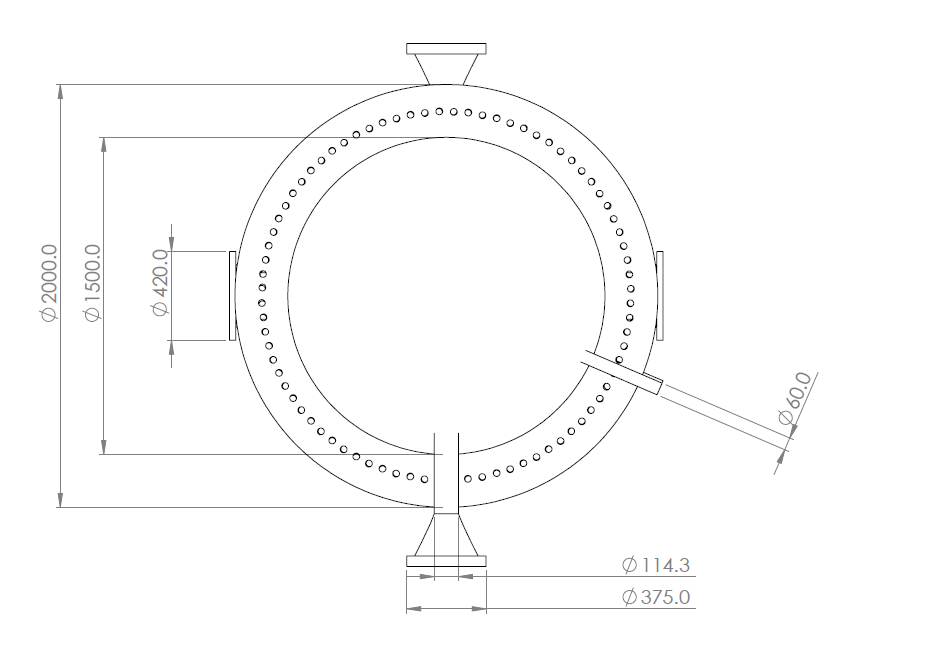
\includegraphics[width=0.6\linewidth]{chapters/2-reaction/figures/FYD reactor bottom view with calc.PNG}
    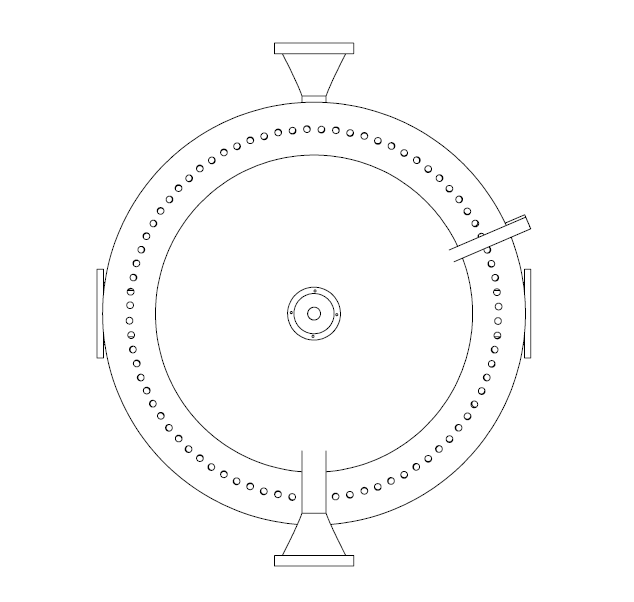
\includegraphics[width=0.45\linewidth]{chapters/2-reaction/figures/FYD reactor top view.PNG}
    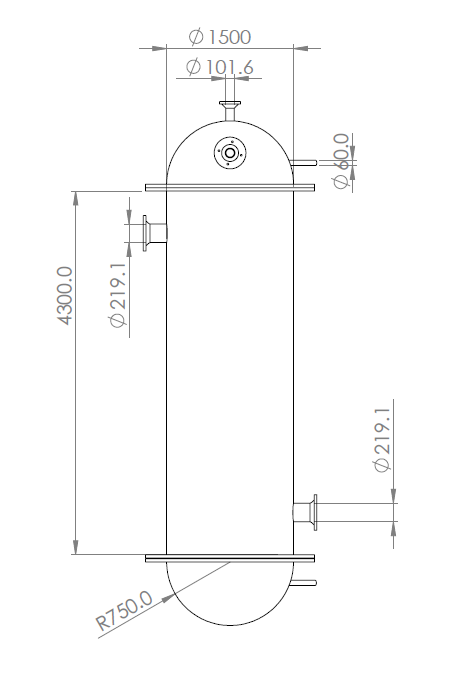
\includegraphics[width=0.49\linewidth]{chapters/2-reaction/figures/FYD reactor right view with calc.PNG}
    \caption{Top, bottom and right view of the reactor. All dimensions in units of mm}
    \label{fig:reactortopbottomrightview}
\end{figure}

\begin{figure}[H]
    \centering

    \begin{subfigure}{0.49\linewidth}
        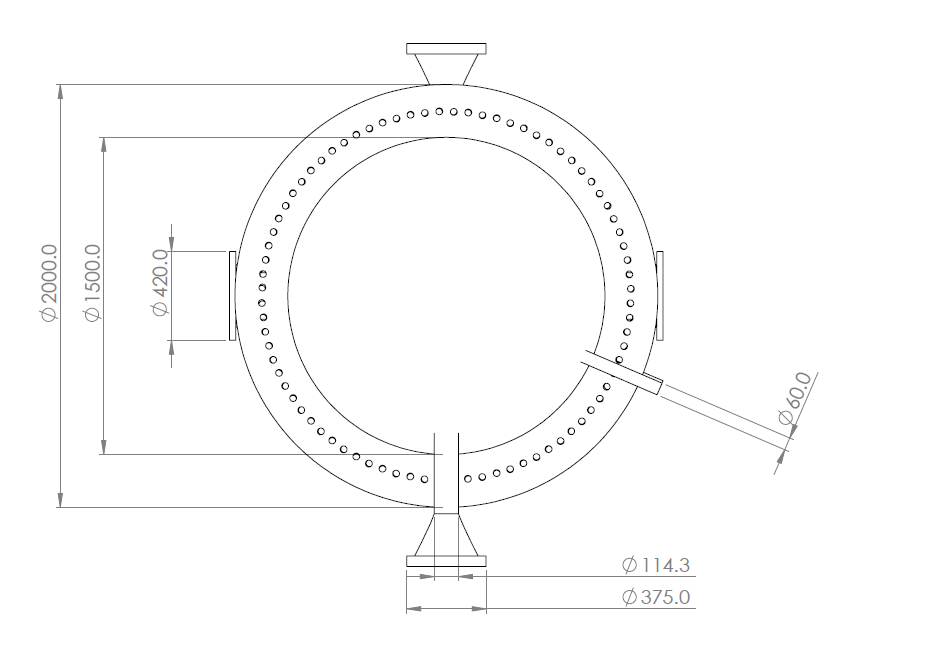
\includegraphics[width=\linewidth]{chapters/2-reaction/figures/FYD reactor bottom view with calc.PNG}
        \caption{Bottom view of the reactor}
        \label{fig:comsol-S2:maxT}
    \end{subfigure}
    \begin{subfigure}{0.49\linewidth}
        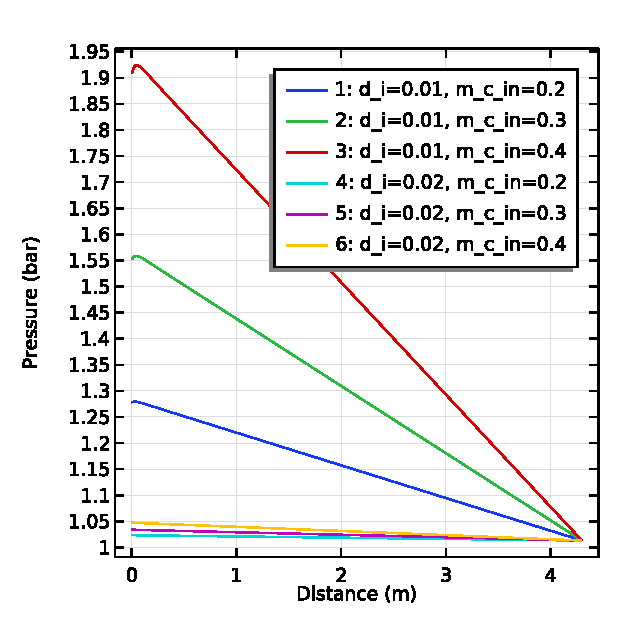
\includegraphics[width=\linewidth]{figures/S2-CW-Pdrop.eps}
        \caption{CW side pressure drop}
        \label{fig:comsol-S2:CW-Pdrop}
    \end{subfigure}

    \caption{Sensitivity to secondary CW parameters}
    \label{fig:comsol-S2}
\end{figure}